\chapter{Framework EPUBKit}
\section{Tworzenie frameworku na iOS}

Tworzenie biblioteki którą zamierzamy następnie wykorzystać we własnej aplikacji lub udostępnić publiczne, jest stosunkowo prostym procesem. Wszystko sprowadza się do stworzenia nowego projektu w Xcode a następnie dołączenie go do przestrzeni roboczej (Xcode Workspace) w której znajdzie się projekt aplikacji nad którą pracujemy oraz projekt biblioteki. Aby stworzyć projekt biblopteki należy uruchomić Xcode IDE i na powitalnym ekranie wybrać opcję "Create a new Xcode project" która przeniesie nas do kolejnego ekranu z możliwością wybrania konktetnego szablonu projektu nad jakim chcemy pracować.

\begin{figure}[ht!]
  \centering
  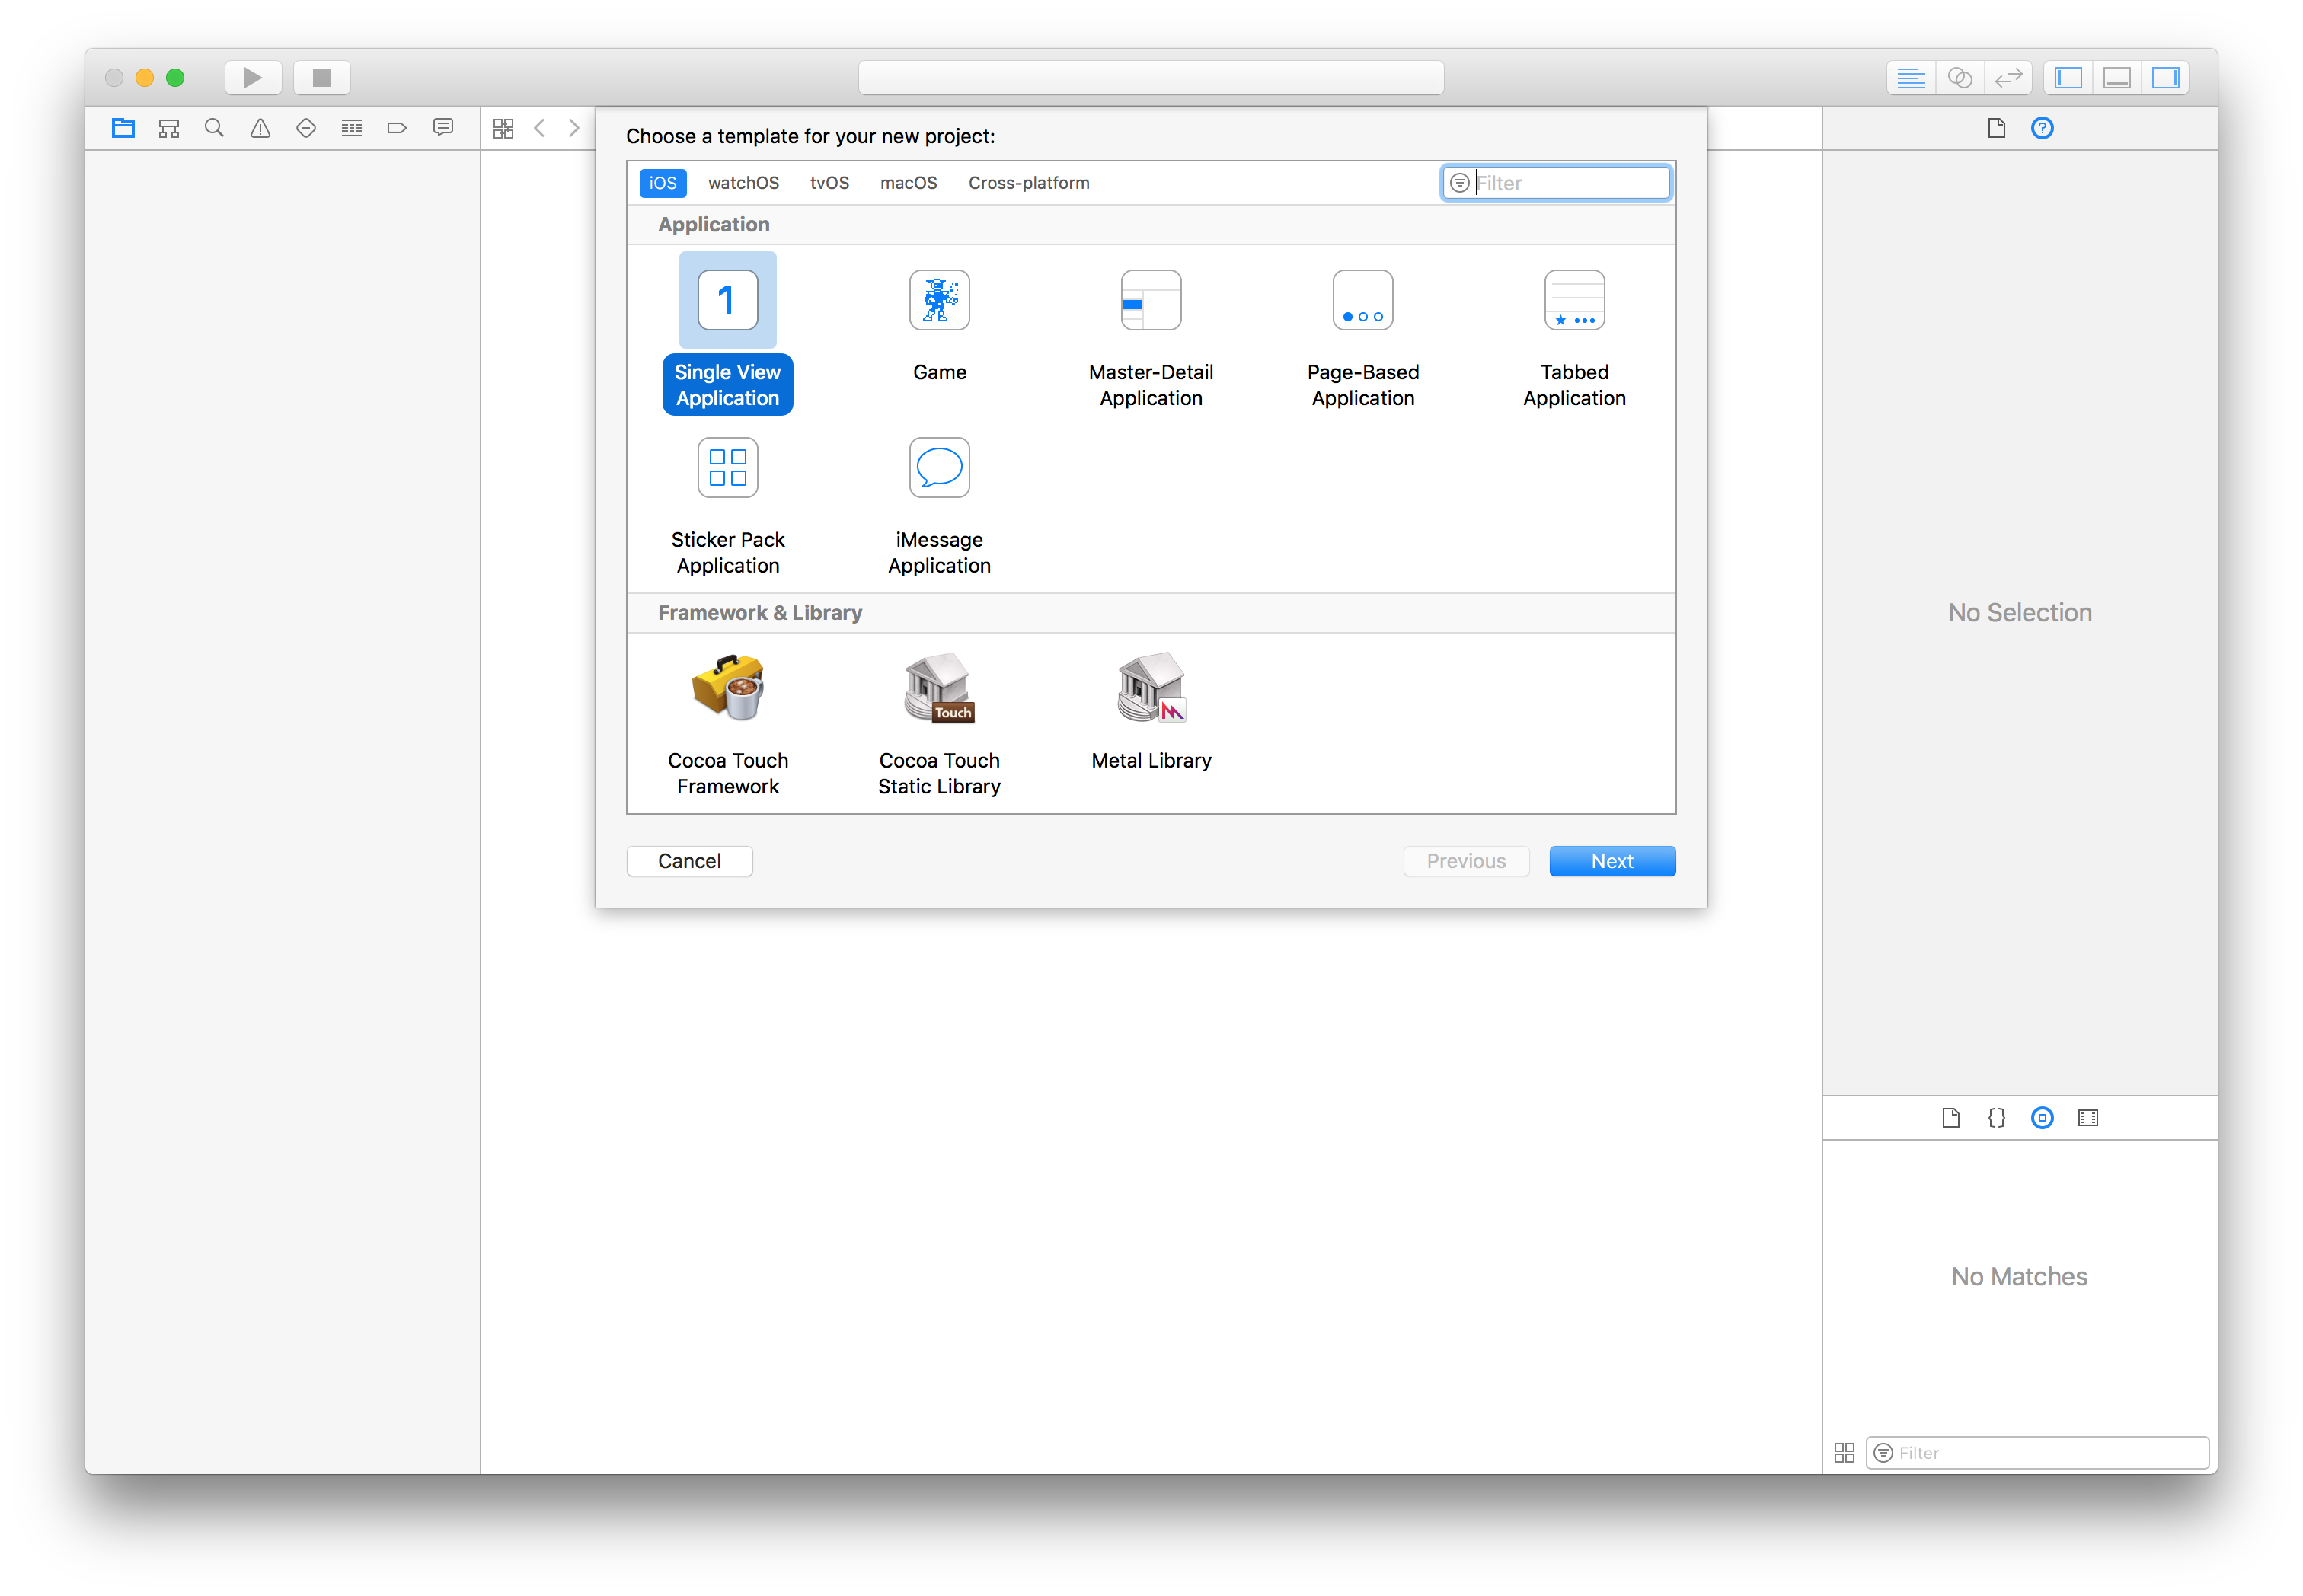
\includegraphics[width=120mm]{images/chapter-4-image-1-new-project.png}
  \caption{Szablny projektów które znajdują się w Xcode}
  \label{chapter-4-image-1-new-project}
\end{figure}

Na naszym przypadku interesuje nas szablon "Cocoa Touch Framework", a po jego wybraniu jesteśmy proszeni o uzupełnienie formularza ze szczegółowymi informacjami na temat projektu który zamierzamy stworzyć, poczynając od nazwy, po język w którym będzie napisany (Swift lub Objective-C). Następnie Xcode poprosi o wskazanie lokalizacji na dysku w której chcemy zapisać projekt oraz zapyta nas czy chcemy stworzy repozytorium systemu kontroli wersji git. W tym momencie mamy projekt który można już w prosty sposób dołączyć do aplikacji (Co zostanie opisane w kolejnym rozdziale przy okazji omawianie wykorzystania biblioteki EPUBKit w demonstracyjnej aplikacji). Teraz już możemy tworzyć klasy które mają składać sie na funkcjonalność biblioteki.

\begin{figure}[ht!]
  \centering
  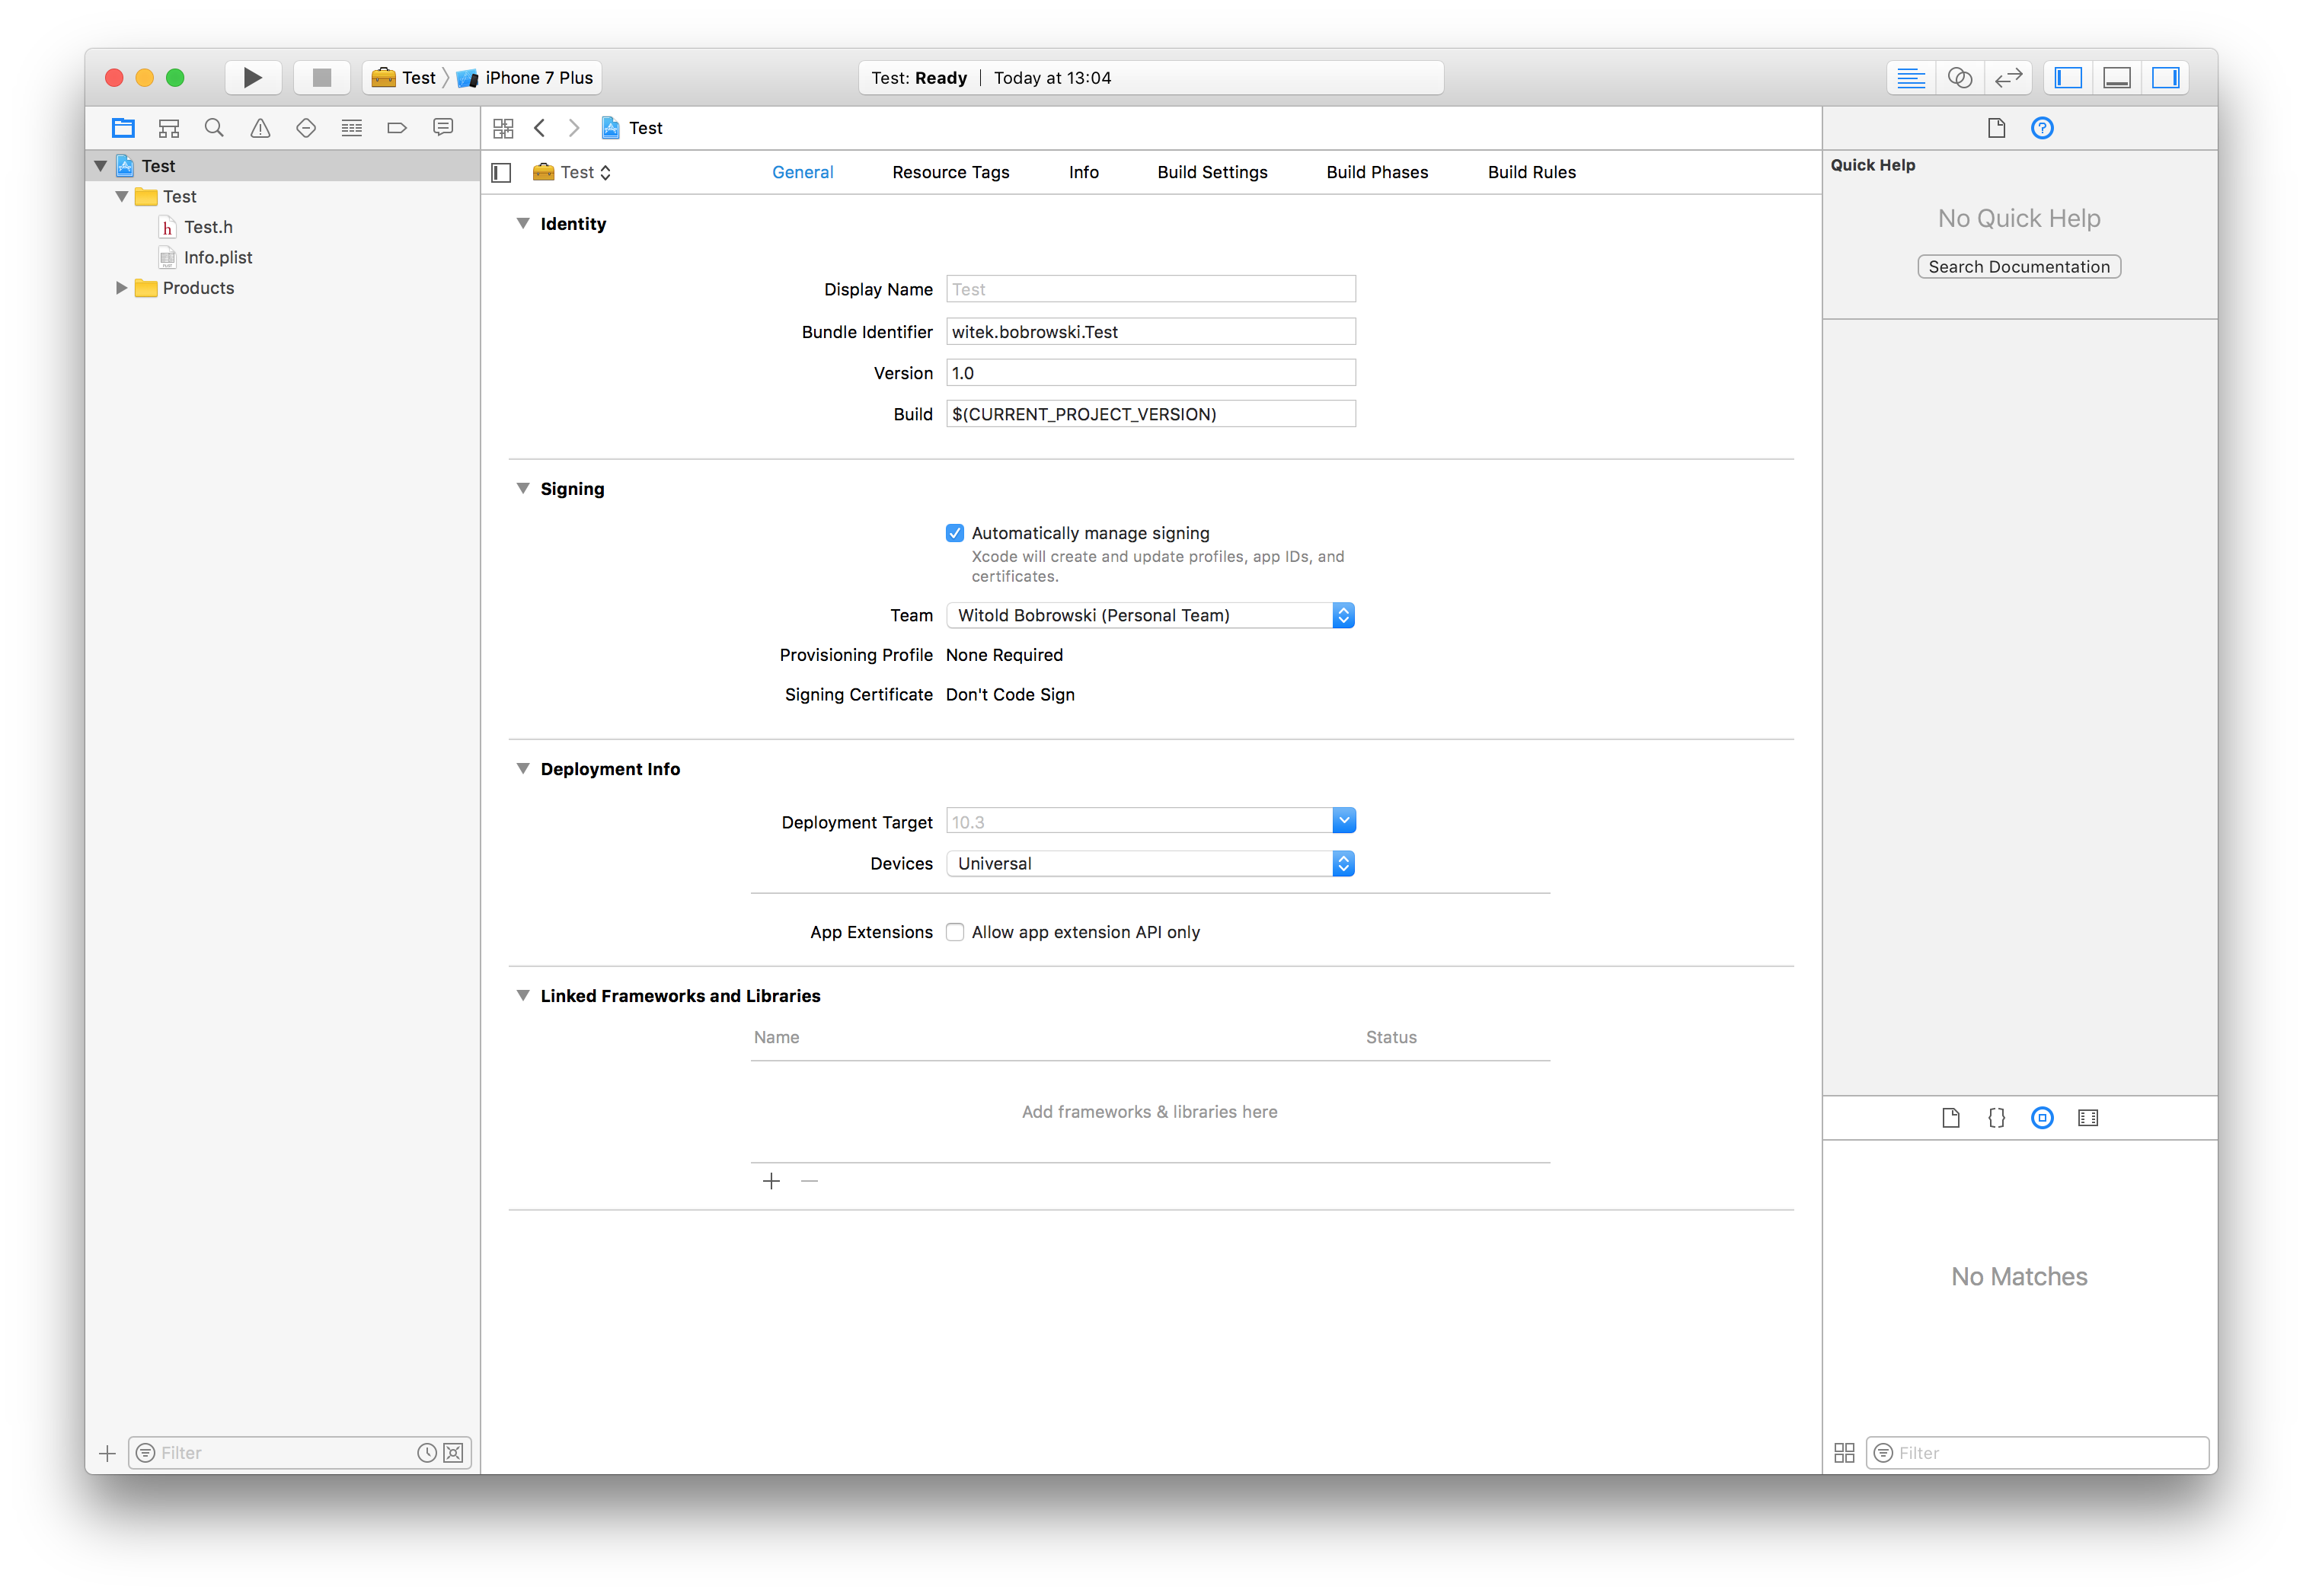
\includegraphics[width=120mm]{images/chapter-4-image-2-empty-project.png}
  \caption{Szablony projektów które znajdują się w Xcode}
  \label{chapter-4-image-2-empty-project}
\end{figure}

Plik projektu pozwala nam za szczegółowy wgląd w preferencje oraz infromacje jego dotyczące, które można zmieniac w dowolnej chwili. Jest możliwość zmiany wersji bibioteki, docelowego urządzenia (iPhone lub iPad), preferowanej wersji systemu który ma wspierać bibltioteka, oraz co bardzo istotne, mamy możliwość użycia innych niezależnych bibliotek w naszym projekcie. Wystarczy wyeksportować plik projektu jako plik przestrzebi roboczej do której można dodać inne projekty a następnie połączyć je z naszym w menu "General" w polu "Linked Frameworks and Libraries" w pliku projektu. Dzięki tak funkcjonalnym i prostym w obsłudze narzędziom jak Xcode, po szybkiej konfiguracji swoją uwagę można skupić na samej logice którą chcemy zaimplementować.

W tym rozdziale zostanie opisana stworzna przez mnie biblioteka EPUBKit. Biblioteka ta jest oparta na architekturze MVC (Model View Controller) dlatego omówienie jest rozpocznę od opisania jej modelu oraz parsera, a następnie przejdę do zawartych w niej widokach które pozwalają na wyświetlenie danych zawartych w modelu. Zakończę rozdział przedstawiając możliwości dystrybuowania takiej biblioteki, przy pomocy szeroko stosowanych i popularnych narzędzi, które są podstawą iOS developmentu.

\section{Model}

Struktura klas modelu została zaprojektowana w ten sposób aby z jednej strony odzwierciedlała struktrę dokumnetu EPUB oraz format OPF który EPUB wykorzystuje, a z drugiej by trzymała się konwencji swiftowych i intuicyjnie reprezontowała obiekt który następnie będzie wykorzystywany w kolejnych klasach biblioteki.

\begin{lstlisting}[caption={Struktura modelu EPUBKit.}, language=bash]
    Model
    |-- EPUBDocument.swift
    |-- EPUBManifest.swift
    |-- EPUBMetadata.swift
    |-- EPUBSpine.swift
    `-- EPUBTableOfContents.swift
\end{lstlisting}

\subsection{EPUBDocument}
\label{EPUBDocument}
EPUBDocumnet jest klasą publiczną reprezentującą całą poblikację EPUB i agregującą pozostałe struktury modelu biblioteki jako jej stałe własności (ze względu na nomenklaturę stosowaną w języku Swift, 'properties' będą nazywane własnościami). W języku Swift odróżniamy dwa rodzaje własności, są to stałe (słowo kluczowe let) do których wartość może zostać przypisana wyłącznie jednokrotnie oraz zmienne (słowo kluczowe var) których wartość może być modyfikowana w dowolnym momencie.

\begin{lstlisting}[caption={Deklaracje własności w Swifcie.\cite{theSwiftProgrammingLanguageDeclarations}}, language=swift-reference]
  let (constant name): (type) = (expression)
  var (variable name): (type) = (expression)
\end{lstlisting}

Własności zostały oznaczone jako stałe ze względu na statyczną naturę struktury publikacji EPUB. Ciężko sobie wyobracić powód dla którego któreś z metadanych publikacji miały by zostać zmienione albo któreś z dokumentów XML usunięte z manifestu publikacji. Dlatego biorąc pod uwagę kontekst, w którym klasa się znajduje, zdecydowałem się oznaczenie jej własności jako stałe aby zapewnić klasie niemodalność oraz zgodność z wytycznymi odnośnie projektowania klas i struktór w języku Swift według których powinno oznaczać się własności jako stałe w każdej sytuacji która nie wymaga od nas ich mutowania, a słowa "mutowania" użyłem tutaj nie bez powodu, co stanie się jasne w kolejnym akapicie.

\begin{lstlisting}[caption={Klasa EPUBDocument i jej stałe publiczne.}, language=swift]
public class EPUBDocument {
    public let directory: URL
    public let contentDirectory: URL
    public let metadata: EPUBMetadata
    public let manifest: EPUBManifest
    public let spine: EPUBSpine
    public let tableOfContents: EPUBTableOfContents
}
\end{lstlisting}

W przeciwieństwie do C, struktury w Swiftcie mogą posiadać metody. W przypadku gdy metoda w jakiś sposób zmiania własności musi ona zostać oznaczona słowem kluczowym 'mutating' co tyczy się również metod enumeracji. Wspominam o tym, ponieważ chciałbym wytłumaczyc dlaczego typy własności klasy EPUBDocument są strukturami a nie klasami. Ze względu na to, że instancje klasy są przekazywane przez referencję, a instancje struktur są przekazywane przez kopiowanie wartości, oznacz to że są one przeznaczone do innych zadań. Zgodnie z wytycznymi Apple, strukturami powinno oznaczać się typy, których zadaniem jest enkapsulacja relatywnie prostych wartości\cite{theSwiftProgrammingLanguageStructsPurpose}, co jest prawdą w przypadku wcześniej wspomnianych typów (zostaną one opisane w kolejnych paragrafach).

Klasa EPUBDocument posiada dwa inicjalizatory które pozwalają tworzyć instancje tej klasy. Pierwszym z nich jest inicjalizator prywatny w nomenklaturze swiftowej "memberwise initializer" ze względu na kolejność argumentów które przyjmuje, która zgodna jest z kolejnością deklajacji własności. Inicjalizator ten został oznaczony jako prywatny ponieważ jego przeznaczeniem jest inicjalizować instancję jedynie przy pomocy drugiego inicjalizatora. Drugi z inicjalizatorów jest dostępny publicznie, i jest jedynym publicznym inicjalizatorem dla tej klasy.

\begin{lstlisting}[caption={Inicjalizatory klasy EPUBDocument.}, language=swift]
private init (directory: URL, contentDirectory: URL, metadata: EPUBMetadata, manifest: EPUBManifest, spine: EPUBSpine, toc: EPUBTableOfContents) {
    self.directory = directory
    self.contentDirectory = contentDirectory
    self.metadata = metadata
    self.manifest = manifest
    self.spine = spine
    self.tableOfContents = toc
}

public convenience init?(named: String) {
    let parser = try? EPUBParser(named: named)
    guard let directory = parser?.directory,
        let contentDirectory = parser?.contentDirectory,
        let metadata = parser?.metadata,
        let manifest = parser?.manifest,
        let spine = parser?.spine,
        let tableOfContents = parser?.tableOfContents else { return nil }
    self.init(directory: directory, contentDirectory: contentDirectory, metadata: metadata, manifest: manifest, spine: spine, toc: tableOfContents)
}
\end{lstlisting}

Zważając na naturę publikacji EPUB jako spójnej całości, zdecydowałem ograniczyć się inicjalizowanie klasy EPUBDocument do inicjalizatora pomocniczego, który wykorzystuje do tego parser. Ten inicjalizator wykorzystuje w pełni możliwości Swifta. Oznaczając go słowem kluczowym "convenience", zmuszam go do wykorzystania wyznaczonego (z ang. designated) inicjalizatora ponieważ pomocniczy inicjalizator nie może samemu tworzyć instancji, musi do tego wykorzystać wyznaczony inicjalizator (w tym przypadku jest to pierwszy inicjalizator, który jest prywatny). Dodatkowo pomocniczy inicjalizator, jest oznaczony znakiem zapytania "init?" co oznacza, że inicjalizacje może się niepowieść, a w takiej sytuacji inicjalizator zwróci... nic, czyli "nil" w Swifcie. Konsekwencją tego jest to, że typ która zwraca ten inicjalizator to "EPUBDocument?" a nie "EPUBDocument", co oznacza że może on nie mieć żadnej wartości co trzeba w odpowiedni sposób obsłużyć. Przeanalizujmy więc krok po kroku operacje, które wykonuje inicjalizator pomocniczy.

\begin{lstlisting}[language=swift-reference]
    let parser = try? EPUBParser(named: named)
\end{lstlisting}

Na wstępie tworzy instancję parsera, i jako argument inicjalizatora podaje własny parametr który wskazuje na nazwę publikacji EPUB. Słowo kluczowe "try" onacza, że inicjalizator może zwrócić błąd, a dzięki znakowi zapytania błąd ten gdy zostanie rzucony, będzie interpretowany jako zwrócenie nila przez inicjalizator. W ten sposób unikamy umieszczenia bloku "do-catch" co znacznie upraszcza kod. Końcowo znajdujemy się w posiadaniu stałej "parser", która jest typu "EPUBParser?" czyli opcjonalny EPUBParser.

\begin{lstlisting}[language=swift-reference]
  guard let directory = ... else { return nil }
\end{lstlisting}

Wyrażenie "guard let" jest jednym ze sposobów obsłużenia typu opcjonalnego. Jest to odmiana wyrażenia "if let" które pozwala nam na przypisanie wartości zmiennej a, do nowej stałej b, jeżeli zmienna a takową posiada. Wadą takiego rozwiązania jest to, że nowo powstała zmienna b, znajduje się jedynie w zasięgu bloku "if", co w pewien sposób ogranicza dostęp do niej. Z pomocą przychodzą wyrażenia "guard", dzięki który zadeklarujemy nową stałą, która będzie przyjmowała wartość zmiennej, którą chcemy "rozpakować" (z ang. unwrap, co odnosi się do czynności wywłaszczania wartości z typu opcjonalnego) i będzie ona dostępna w obrębie tego samego bloku co wyrażenie guard. Dodatkowo mamy możliwość wykonania jakiejść czynności w sytuacji gdy zmienna którą rozpakowywujemy nie ma wartości, co w tym konkretnym przypadku będzie oznaczało niepowodzenie wywłaszczenia którejś z wartości parsera a więc inicjalizator EPUBDocument zwróci nil. Ponieważ wyrażenie "guard" działa w podobny sposób co "if", otrzymuje on również te same funkcjonalności co "if" w Swifcie, czyli możliwość kolejkowania wyrażeń zwracających wartość boolowską (wypisujemy je kolejno po przecinku), i w przypadku zwrócenia fałszu przez jedno z nich, instrukcja natychmiast zostaje przerwana a pozostałe wyrażenia nie zostają ewaluowane, a w tym przypadku program przechodzi do bloku "else".

\begin{lstlisting}[language=swift-reference]
    self.init(...)
\end{lstlisting}

Jeżeli udało się wywłaszczyć wszystkie potrzebne wartości z parsera, to można przejść do tworzenia instancji EPUBDocument. Inicjalizator pomocniczy wywołuje inicjalizator wyznaczony, i dokument zostaje pomyślnie stworzony a wszystkie informacie otrzymane dzięki parserowi zostają przypisane na stałe do jednej instancji EPUBDocument. W ten sposób zostaje zachowana niemutowalność instancji, oraz gwarancja, że wszystkie wartości w których posiadaniu znajduje się instancja, pochodzą z jednego źródła, z którego czerpie parser. Działanie samego parsera zostawiam na kolejny podrozdział.

\subsection{EPUBManifest}

Jak juz wspomniano w rozdziale opisującym format EPUB, jego struktura jest oparta o standard OPF a to oznacza, że znajduję się w nim wykaz (manifest) wszystkich dokumentów oraz zasobów na które składa się dokument. Każdy element wymieniony w manifescie posiada swoje ID, wskazaną ścieżke w strukturze dokumentu oraz typ (Media Type). Parser starannie analizuje manifest i tworzy strukturę w której posiadaniu następnie znajduje się instancja EPUBDocument o czym więcej przy okazji omawiania parseru.

\begin{lstlisting}[caption={Struktura EPUBManifest.}, language=swift]
public struct EPUBManifest {
    public struct Item {
        public var id: String
        public var path: String
        public var mediaType: EPUBMediaType
        public var property: String?
    }

    public var id: String?
    public var items: [String:Item]

    public func path(forItemWithId id: String) throws -> String {
        if let item = items[id] {
            return item.path
        } else {
            throw EPUBParserError.noPathForItem(id)
        }
    }
}
\end{lstlisting}

EPUBManifest deklaruje własną strukturę Item, na którą skłda się kilka własności opisujących daną pozycję w manifescie. EPUBManifest posiada dwie własniości. Pierwszą z nich jest opcjonane ID manifestu które może się pojawić w publikacji EPUB, ale w specyfikacji nie jest określone jako wymagane pole. Drugą własnością jest słownik, którego kluczem jest ID elementu a wartością jest instancja struktury Item. Ponieważ manifest nie musi być listą posortowaną, zdecydowałem się na użycie słownika jako struktury danych która ma przechowywać wszystkie jego elementy, dzięki czemu dostęp do nich jest natychmiastowy. Należy zwrócić uwagę na to, że nie został zadeklarowany inicjalizator dla EPUBManifest, tak jak miało to miejsce przy EPUBDocument. Powód jest następujący, Swift w przypadku gdy żaden inicjalizator nie został zadeklarowany dostarcza domyślny "memberwise initializer" dzięki czemu w EPUBManifest dostajemy go "za darmo", natomist w przypadku struktury EPUBDocument został zadeklarowany pomocniczy inizjalizator przez co domyślny inicjalizator nie został dostarczony przez swift. EPUBManifest posiada publiczną metodę która przyjmuje jako argument id elementu zwraca do niego ścieżkę w przypadku gdzy element znajduje się w słowniku "items". Słownik w swifcie zwraca wartość o typie opcjonalnym, ponieważ nie ma żadnej gwarancji, że do podanego przez nas kluczu przypisana jest jakaś wartość. Zastosowano tutaj rozpakowanie typu opcjonalnego przy pomocy wyrażenia "if let" aby otrzymać ścieżkę elementu. W przypadku gdy znaduje się on w słowniku zostanie on przypisany do nowej stałej której typ już nie jest opcjonalny więc posiadanie przez niej jakiejś wartości jest zagwarantowane. Dodatkowo w przypadku gdyby taki element manifestu o wskazanym ID nie istniał, zostanie rzucny błąd co zostało oznaczone słowem kluczowym "throws" przy deklaracji zwracanego typu.

\begin{lstlisting}[caption={Funkcje i metody które mogą rzucać błędy, przy deklaracji muszą zostać oznaczone słowem kluczowym "throws"\cite{theSwiftProgrammingLanguageDeclarations}.},language=swift-reference]
func (function name)((parameters)) throws -> (return type) {
    (statements)
}
\end{lstlisting}

W kontekście EPUBManifest pozostało jeszcze wspomnieć o typie enumeracji, który został stworzony aby określać charakter elementu znajdującego się w publikacji EPUB, i wymienionego w Manifescie. Mowa tutaj o EPUBMediaType, enumeracji która posiada powiązany typ (Associated Type) którym jest typ String.

\begin{lstlisting}[caption={Enumeracja EPUBMediaType.}, language=swift]
public enum EPUBMediaType: String {
    case gif = "image/gif"
    case jpeg = "image/jpeg"
    case png = "image/png"
    case svg = "image/svg+xml"
    case xHTML = "application/xhtml+xml"
    case rfc4329 = "application/javascript"
    case opf2 = "application/x-dtbncx+xml"
    case openType = "application/font-sfnt"
    case woff = "application/font-woff"
    case mediaOverlays = "application/smil+xml"
    case pls = "application/pls+xml"
    case mp3 = "audio/mpeg"
    case mp4 = "audio/mp4"
    case css = "text/css"
    case woff2 = "font/woff2"
    case unknown
}
\end{lstlisting}

Enumeracja ta deklaruje wszystkie przypadki typu mediów wspieranych przez standard EPUB i wymienionych w specyfikacji. Dzięki tej enumeracji element manifestu posiada własność które jest ograniczona do kilku przypadków, a w sytuacji potrzeby obslużenia takiego elementu w prosty sposób można zdeterminować jego rodzaj. Powiązana wartość dla każdego przypadku jest ciągiem znaków reprezentującym typ określony w specyfikacji EPUB, i gwarantuje nam ona prostą inicjalizację przez podanie wartości jako argument inicjalizatora enumeracji.

\subsection{EPUBMetadata}

Kolejny elementem wymaganym przez OPF jest metadata, który enkapsuluje meta informacje na temat konkretnej interpretacji zawartej w publikacji. W celach reprezentacji tych meta danych w bibliotece EPUBKit została swtorzona struktura EPUBMetadata.

\begin{lstlisting}[caption={Struktura EPUBMetadata.}, language=swift]
public struct EPUBMetadata {
    public struct Creator {
        public var name: String?
        public var role: String?
        public var fileAs: String?
    }
    public var contributor: Creator?
    public var coverage: String?
    public var creator: Creator?
    public var date: String?
    public var description: String?
    public var format: String?
    public var identifier: String?
    public var language: String?
    public var publisher: String?
    public var relation: String?
    public var rights: String?
    public var source: String?
    public var subject: String?
    public var title: String?
    public var type: String?
    public var coverId: String?
}
\end{lstlisting}

EPUBMetadata definiuje własny publiczny typ pomocniczy Creator aby w lepszy sposób reprezentować element twórcy i wspołtwórcy publikacji którzy mogą zostać wymienieni w meta danych publikacji EPUB. Wszystkie własności EPUBMetadata posiadają typ opcjonalny, ponieważ ich obecność w dokumencie EPUB nie jest zagwarantowana. Inicjalizator nie jest obecny, ponieważ po raz kolejny jest dostarczony domyslny inicjalizator przez Swift. Własności są oznaczone jako zmienne publiczne, ponieważ udostępnienie ich globalnie ma sens ze względu na ich informatywny cel. Własność metadata w klasie EPUBDocument jest stałą, a więc pomimo tego iż w deklaracji struktury EPUBMetadata jej własności są zmiennymi, to w momencie przypisania jej instancji do instancji klasy EPUBDocument wartości zmiennych nie mogą zostać zmienione, co wynika z natury struktury w swiftcie która jest kopiowana przez wartość. Mutowanie wartości zmiennych w instancji struktury EPUBMetadata, która nie znajduje się w kontekście całego dokumentu, ma sens a przynajmniej nie jest niedopuszczalne. W przypadku gdyby parser znajdujący się w posiadaniu takiej instancji, w pewnym momencie wywłaszczył pewne dodatkowe dane z dokumentu, warto pozwolić mu na uaktualnienie ich w strukturze. Niemutowalność zostaje zagwarantowana dopiero w momencie przypisania jej jako stałej w klasie EPUBDocument.

\subsection{EPUBSpine}

Element "spine" w publikacji EPUB definiuje kolejność w jakiej elementy manifestu są uporządkowane, czyli w jakiej kolejności należy je wyświetlać. Element ten znajduje swoją reprezentację w bibliotece EPUBKit, jako struktura EPUBSpine.

\begin{lstlisting}[caption={Struktura EPUBSpine.}, language=swift]
public struct EPUBSpine {
    public struct Item {
        public var id: String?
        public var idref: String
        public var linear: Bool
    }

    public var id: String?
    public var toc: String?
    public var pageProgressionDirection: EPUBPageProgressionDirection?
    public var items: [Item]
}
\end{lstlisting}

EPUBSpine podobnie do EPUBManifest deklaruje własny typ pomocniczy Item, które odzwierdziedla "itemref" znajdujący się w "spine" publikacji EPUB. Item posiada własności które odnoszą się do identyfikatora elementu manifestu (idref), dodatkowego indentyfikatora, oraz istotnej informaci, czy element powinien zostać wyświetlony w kolejności liniowej, czy nie. Struktura EPUBSpine składa się z pola "id", "toc" które opcjonalnie może posiadać identyfikator spisu treści jeżeli takowy się znajduje w dokumencie, własności która definiuje kierunek w którym powinno się wyświetlać elementy dokumentu, oraz tablicę elementów własnego typu Item.

\begin{lstlisting}[language=swift]
public enum EPUBPageProgressionDirection: String {
    case leftToRight = "ltr"
    case rightToLeft = "rtl"
}
\end{lstlisting}

Zmienna "pageProgressionDirection" posiada typ który został zadeklarowany przeze mnie jako enumeracja EPUBPageProgressionDirection składająca się z dwóch przypadków, pierwszego który reprezentuje kolejność czytania od lewej do prawej oraz drugiego, który mówi o kierunku przeciwnym. W przypadku gdy kolejność nie zostanie zdefiniowana w publikacji, decyzja jak dokument powinien zostać wyswietlony zostaje pozostawiona systemowi czytającemu. W celu szybkiej inicjalizacji i zdefiniowaniu odpowiedniego kierunku dzieki powiązanemu typowi, parser podaje jako argument inicjalizatora enumeracji wartość która wywłaszczył z publikacji EPUB, która przyjmuje wartość "rtl" lub "ltr".

\subsection{EPUBTableOfContents}

Ostatnia struktura modelu reprezentuje spis treści zawarty w publikacji EPUB. Pomimo tego iż w wersji trzeciej standardu nie jest wspierany w takiej formie jak w poprzednich wersjach, to ze wzgledu na zapewnienie wsparcia tym starszym wersjom publikacji zdecydowałem się zaimplementować tą relatywnie prostą strukturę. Spis treści przedstawiony w formie pliku typu NCX służył w poprzednich wersjach EPUB użytkownikowi do nawigacji w obrębie dokumentu, jednak specyfikacja wymaga od systemu czytającego ignorowania tego pliku w publikacjach wersji trzeciej.

\begin{lstlisting}[caption={Struktura EPUBTableOfContents.}, language=swift]
public struct EPUBTableOfContents {
    public var label: String
    public var id: String
    public var item: String?
    public var subTable: [EPUBTableOfContents]?
}
\end{lstlisting}

EPUBTableOfContents posiada własności które znamy już z poprzednich struktur, jednakże to co ją od nich wyróżnia to możliwość zagnieżdzenia. Ponieważ rozdziały mogą posiadać podrozdziały, a te z kolei mogą być podzielone na jeszcze mniejsze części, co może zostać uwzlędnione w takim spisie treści, konieczne jest pozwolenie przechowywania przez każdą pozycje swojej własnej tablicy. A skoro sam spis posiada takie same atrybuty co jej elementy, postanowiłem nie tworzyć dodatkowej struktury Item jak we wcześniej omówionych strukturach. Swift zapewnia nam domyślny inizjalizator więc po raz kolejny unikamy konieczności implementowania go ręcznie.

\section{Parser}

Pierwotnie planowałem opisać Parser w rozdziale poświęconym modelowi, ponieważ w architekturze MVC bibliteki EPUBKit jego rolna mocno wpasowywuje się w definicję modelu, ponieważ to własnie on go tworzy. Jednakże zdecydowałem, że rozsądniej będzie gdy przeznacze na to osobny podrozdział ze względu na to jak obszerny jest to temat ze względu na jego architekturę, oraz ilość wykonywanych operacji.

\begin{lstlisting}[caption={Struktura folderu narzędzi służacych modelowi EPUBKit.}, language=bash]
  Utils
  |-- EPUBParsable.swift
  |-- EPUBParser.swift
  `-- EPUBParserError.swift
\end{lstlisting}

\subsection{EPUBParsable}

Aby praca parsera była dobrze zorganizowana, zdecydowałem się zaimplementować wzorzec projektory Budowniczy (ang. Buildier), ponieważ jest on zgodny z naturą parsera, który wywłaszcza informacje z publikacji EPUB a następnie na ich podstawie buduje model EPUBKit którym jest EPUBDocument. Pierwszym krokiem w celu zaimplementowania wzorcu Budowniczego było stworzenie protokołu, który zostanie zastosowany przez parser.

\begin{lstlisting}[caption={Protokół EPUBParsable.}, language=swift]
protocol EPUBParsable {
    func unzip(archive name: String) throws -> URL
    func getContentPath(from bookDirectory: URL) throws -> URL
    func getMetadata(from xmlElement: AEXMLElement) -> EPUBMetadata
    func getManifest(from xmlElement: AEXMLElement) -> EPUBManifest
    func getSpine(from xmlElement: AEXMLElement) -> EPUBSpine
    func getTableOfContents(from xmlElement: AEXMLElement) -> EPUBTableOfContents
}
\end{lstlisting}

Protokół ten deklaruje metody, które każda stosująca go klasa lub struktura będzie musiała zaimplementować. Konwencja nazewnictwa protokołów w swifcie jest taka, aby nazywać je tak aby dobrze określały naturę klasy którą go stosuje, aby pasowały do cech które nadają klasom. Jeżeli protokół opisuje czym klasa jest, to powinien być czytany jako rzeczownik jak np. protokół standardowej biblioteki swifta MutableCollection. Protokoły, które opisują funkcjonalność, pewne dodatkowe możliwości powinny być kończyć się -ible lub -able. Dzięki tej konwencji, odrazu staje się jasne jakich cech nabywa klasa juz w momencie oznaczenia że stosuje ona dany protokół. Zaimplementowanie przez stosującą protokół klasę jego metod jest wymagane, ponieważ na ten moment nie istnieje żadna implementacja domyślna. Swift pozwala na dostarczenie tak zwanych rozszeżeń deklarowanych typów przy pomocy słowa kluczowego "extension". Dzięki tym rozszerzeniom deklarację typu można podzielić na schludnie wyglądające i dobrze zorganizowne bloki kodu, co zostanie przedstawione przy omawianiu klasy EPUBParser.

\begin{lstlisting}[caption={Deklaracja wyrażenia "extension"\cite{theSwiftProgrammingLanguageDeclarations}.},language=swift-reference]
extension (type name): (adopted protocols) {
    (declarations)
}
\end{lstlisting}

Takie rozszeżenie można wykorzystać również w protokołach (które są typem tak samo jak klasa czy struktura), i dostarczyć im domyślną implementacje metody lub zadeklarować nowe. Jednakże w tym przypadku nie będę tego robił ze względu na to iż EPUBParser powinien zaimplementować każdą z nich w kontekście konkretnego dokumentu.

\subsection{EPUBParser}

Zadaniem parsera jest zebranie wszystkich informacji na temat publikacji i enkapsulacji ich w zmienncyh o typach które posiada EPUBDocument, i pełni rolę budowniczego. Jego deklaracja to zbiór właściwości o typie opcjonalnym oraz inicjalizator, w którym odbywa się cały proces budowania modelu, poprzez parsowanie publikacji EPUB.

\begin{lstlisting}[caption={Klasa EPUBParser.}, language=swift]
class EPUBParser {
    var directory: URL?
    var contentDirectory: URL?
    var metadata: EPUBMetadata?
    var manifest: EPUBManifest?
    var spine: EPUBSpine?
    var tableOfContents: EPUBTableOfContents?

    init(named: String) throws {
        do {
            directory = try unzip(archive: named)
            let contentPath = try getContentPath(from: directory!)
            contentDirectory = contentPath.deletingLastPathComponent()
            let data = try Data(contentsOf: contentPath)
            let content = try AEXMLDocument(xml: data)
            metadata = getMetadata(from: content.root["metadata"])
            manifest = getManifest(from: content.root["manifest"])
            spine =  getSpine(from: content.root["spine"])
            let tocPath = contentDirectory!.appendingPathComponent(try manifest!.path(forItemWithId: spine?.toc ?? ""))
            let tocData = try Data(contentsOf: tocPath)
            let tocContent = try AEXMLDocument(xml: tocData)
            tableOfContents = getTableOfContents(from: tocContent.root)
        } catch {
            print(error.localizedDescription)
            throw error
        }
    }
}
\end{lstlisting}

W przeciwieństwie do wcześniej zadeklarowanych typów, EPUBParser tak jak i protokół EPUBParsable, nie są oznaczone jako publiczne, więc nie mogą zostać użyte poza biblioteką. Domyślnym parametrem dostępu w Swifcie jest "internal", który ogranicza typ, czy właściwość do użytku w obrębie jednego projektu, w tym przypadku biblioteki. Powodem tego jest sposób w jaki zorganizowana została inizjalizacja EPUBDocument. Osobie z zewnątrz najprawdopodobniej nie zależy aby się dowiedzieć w jaki sposob powstaje instancja dokumentu, dla niej ważne jest to, że może otrzymać ją podając jako argument inicjalizatora nazwę pliku, a cały proces będzie odbywał się poza jego zasięgiem. EPUBParser odgrywa tutaj rolę budowniczego, i w momencie rozpoczęcia inicjalizacji dokumentu jego własna instancja zostaje stworzona i "oddelegowana" do wykonania zadania do którego jest przeznaczona. Klasa EPUBParser nie ma innego zastosowania, i nie ma absolutnie żadnego powodu aby używać jej niezależnie i do innych celów niż ten jeden, z góry narzucony. Dlatego też ani klasa, ani jej własności nie są oznaczone publicznymi. Warto zwrócić uwagę na to, iż w swojej deklaracji EPUBParser nie stosuje protokołu EPUBParsable, co wynika ze stylu i wytycznych apple odnośnie projetkowania klas. Klasa powinna deklarować to co dla niej najbardziej elementarne, a dopiero przy użyciu "extension" funkcjonalność powinna zostawać do niej dodawana. I tak jest w tym przypadku, gdzie zadeklarowane są zmienne oraz inicjalizator który już wykonuje metody których jeszcze są dla niego nie znane, a zostaną dopiero zaimplementowane po zastosowaniu protokołu.

\begin{lstlisting}[caption={Klasa EPUBParser stosuje protokół EPUBParsable.}, language=swift]
//MARK: - EPUBParsable
extension EPUBParser: EPUBParsable {
    func unzip(archive named: String) throws -> URL { ... }
    func getContentPath(from bookDirectory: URL) throws -> URL { ... }
    func getMetadata(from content: AEXMLElement) -> EPUBMetadata { ... }
    func getManifest(from content: AEXMLElement) -> EPUBManifest { ... }
    func getSpine(from content: AEXMLElement) -> EPUBSpine { ... }
    func getTableOfContents(from toc: AEXMLElement) -> EPUBTableOfContents { ... }
}
\end{lstlisting}

Dobrą praktyką jest dołączenie komentarzu przy każdym rozszeżeniu aby oznaczyć dodatkowo co oferuje dane rozszeżenie. Należy również pamiętać aby dla każdego stosowanego protokołu przeznazcyć osobne rozszeżenie w celu zwięszenia czytelności kodu. Omówię teraz, krok po kroku w jaki sposób postępuje inicjalizacja parsera, i w jaki sposób wywłaszcza on dane z publikacji w formacie EPUB prezentując kod implementacji każdej z metod protokołu.

\begin{lstlisting}[language=swift-reference]
  init(named: String) throws {
      do {
          ...
      } catch {
          print(error.localizedDescription)
          throw error
      }
  }
\end{lstlisting}

Inicjalizator przyjmuje jako argument nazwę pliku publikacji, i składa się bloku do-catch w którym odbywa się parsowanie. W przypadku gdy któraś z metod rzuci błąd, zostanie on rzucony dalej i zostanie wyświelnona na konsoli informacja o błędzie, który został napotkany. Błędy, które mogą zostać rzucone są typu EPUBParserError, który zostanie omówiony pod koniec podrozdziau dotyczącego parsera. Przejdźmy zatem do instrukcji znajdujących się w bloku do-catch.

\begin{lstlisting}[firstnumber=11, language=swift]
    directory = try unzip(archive: named)
\end{lstlisting}

Pierwszą czynnością parsera jest rozpakowanie archiwum .epub, które w rzeczywistości jest archiwum w stylu ZIP, co omówiono dokładnie w rozdziale trzecim. Dzięki wykorzystaniu open-sourcowej biblioteki ZIP, proces jest ten wyjątkowo prosty.

\begin{lstlisting}[caption={Implementacja metody unzip(archive named:).},language=swift-reference]
    func unzip(archive named: String) throws -> URL {
        Zip.addCustomFileExtension("epub")
        do {
            let filePath = Bundle.main.url(forResource: named, withExtension: "epub")!
            let unzipDirectory = try Zip.quickUnzipFile(filePath)
            return unzipDirectory
        } catch ZipError.unzipFail {
            throw EPUBParserError.unZipError
        }
    }
\end{lstlisting}

W pierwszej kolejności metoda dodaje do klasy Zip rozszerzenie ".epub" aby bilbioteka rozpoznała plik jako archiwum. Następnie w bloku do-catch dochodzi do ustalenia lokalizacji pliku w paczce aplikacji oraz rozpakowania archiwum metodą, która zwraca ścieżkę do docelowego folderu, w którym znajduje się rozpakowana publikacja EPUB. Jeżeli proces rozpakowania przebiegnie bezbłędnie, metoda zwróci ścieżkę.

\begin{lstlisting}[firstnumber=12, language=swift]
    let contentPath = try getContentPath(from: directory!)
    contentDirectory = contentPath.deletingLastPathComponent()
\end{lstlisting}

Inicjalicator wywołuje następnie metodę, która lokalizuje w publikacji obowiązkowy plik "content.opf" w folderze "META-INF" a następnie szuka w nim elementu "rootfile", który jest plikiem OPF, opisującym zawartość całej publikacji.

\begin{lstlisting}[caption={Implementacja metody getContentPath(from bookDirectory:).},language=swift-reference]
    func getContentPath(from bookDirectory: URL) throws -> URL {
        do {
            let path = bookDirectory.appendingPathComponent("META-INF/container.xml")
            let data = try Data(contentsOf: path)
            let container = try AEXMLDocument(xml: data)
            let content = container.root["rootfiles"]["rootfile"].attributes["full-path"]
            return bookDirectory.appendingPathComponent(content!)
        } catch {
            throw EPUBParserError.containerParseError
        }
    }
\end{lstlisting}

Po raz kolejny instrukcje metody znajdują się w bloku do-catch aby zapewnić obsługę ewentualnych błędów. W przypadku zlokalizowania pliku OPF, ścieżka do niego zostaje zwrócona a w przeciwnym wypadku, zostanie rzucony błąd. Jeżeli funkcja zwróci ścieżkę pliku OPF, inicjalizator przypisze do zmiennej "contentDirectory" ściężkę do folderu w którym się on znajduje przez usunięcie ostatniego komponentu ściezki.

\begin{lstlisting}[firstnumber=14, language=swift]
        let data = try Data(contentsOf: contentPath)
        let content = try AEXMLDocument(xml: data)
\end{lstlisting}

Znając już lokalizację pliku OPF, należy go sparsować przy użyciu zewnętrzenej biblioteki AEXML. Dzięki temu dostęp do elemnetów dokumentu będzie znacznie uproszczony, dokument zostanie przedstawiony w formie klasy AEXMLDocument. Jeżeli próba inicjalizacji klas Data oraz AEXMLDocument przebiegnie poprawnie, otrzymamy zmienna "content", z której parser będzie wywłaszczał kluczowe infromacje dotyczące dokumentu.

\begin{lstlisting}[firstnumber=16, language=swift]
        metadata = getMetadata(from: content.root["metadata"])
        manifest = getManifest(from: content.root["manifest"])
        spine =  getSpine(from: content.root["spine"])
\end{lstlisting}

Inicjalizator gdy znajdzie się w posiadaniu dokumentu OPF w formie dokumentu AEXMLDocument, będzie następnie podawał jako argumenty odpowiednim funkcjom jego elementy.

\begin{lstlisting}[caption={Implementacja metody getMetadata(from xmlElement:).},language=swift-reference]
    func getMetadata(from xmlElement: AEXMLElement) -> EPUBMetadata {
        var metadata = EPUBMetadata()
        metadata.contributor = EPUBMetadata.Creator(name: content["dc:contributor"].value,
                                       role: content["dc:contributor"].attributes["opf:role"],
                                       fileAs: content["dc:contributor"].attributes["opf:file-as"])
        metadata.coverage = content["dc:coverage"].value
        metadata.creator = EPUBMetadata.Creator(name: content["dc:creator"].value,
                                   role: content["dc:creator"].attributes["opf:role"],
                                   fileAs: content["dc:creator"].attributes["opf:file-as"])
        metadata.date = content["dc:date"].value
        metadata.description = content["dc:description"].value
        metadata.format = content["dc:format"].value
        metadata.identifier = content["dc:identifier"].value
        metadata.language = content["dc:language"].value
        metadata.publisher = content["dc:publisher"].value
        metadata.relation = content["dc:relation"].value
        metadata.rights = content["dc:rights"].value
        metadata.source = content["dc:source"].value
        metadata.subject = content["dc:subject"].value
        metadata.title = content["dc:title"].value
        metadata.type = content["dc:type"].value
        for metaItem in content["meta"].all! {
            if metaItem.attributes["name"] == "cover" {
                metadata.coverId = metaItem.attributes["content"]
            }
        }
        return metadata
    }
\end{lstlisting}

Działanie metody agregującej meta dane jest relatywnie proste, musi ona przeanalizować elementy zawarte w przekazanej instancji AEXMLElement. Elementy te są oznaczone w sposób określony w specyfikacji, więc nazwane onę będa zawsze w ten sam sposób co znacznie upraszcza proces budowy instancji EPUBMetadata.

\begin{lstlisting}[caption={Implementacja metody getManifest(from xmlElement:).},language=swift-reference]
    func getManifest(from xmlElement: AEXMLElement) -> EPUBManifest {
        var items: [String:EPUBManifest.Item] = [:]
        for item in xmlElement["item"].all! {
            let id = item.attributes["id"]!
            let path = item.attributes["href"]!
            let mediaType = item.attributes["media-type"]
            let properties = item.attributes["properties"]
            items[id] = EPUBManifest.Item(id: id, path: path, mediaType: EPUBMediaType(rawValue: mediaType!) ?? .unknown, property: properties)
        }
        return EPUBManifest(id: xmlElement["id"].value, items: items)
    }
\end{lstlisting}

Metoda "getManifest(from content:)" w pierwszej kolejności tworzy instancję słownika, który znamy ze struktury EPUBManifest. reprezentuje on wszystkie elementy wymienione w manifeście. Następnie iteruje po tablicy elementów zawartych w parametrze "xmlElement", i inicjalizuje przy każdym z nich nową instancję struktury EPUBManifest.Item z informacji, które udało jej się wywłaszczyć.

\begin{lstlisting}[caption={Implementacja metody getSpine(from xmlElement:).},language=swift-reference]
    func getSpine(from xmlElement: AEXMLElement) -> EPUBSpine {
        var items: [EPUBSpine.Item] = []
        for item in xmlElement["itemref"].all! {
            let id = item.attributes["id"]
            let idref = item.attributes["idref"]!
            let linear = (item.attributes["linear"] ?? "yes") == "yes" ? true : false
            items.append(EPUBSpine.Item(id: id, idref: idref, linear: linear))
        }
        let pageProgressionDirection = xmlElement["page-progression-direction"].value ?? ""
        return EPUBSpine(id: xmlElement.attributes["id"], toc: xmlElement.attributes["toc"], pageProgressionDirection: EPUBPageProgressionDirection(rawValue: pageProgressionDirection), items: items)
    }
\end{lstlisting}

W identycznym stylu działa metoda "getSpine(from content:)", kórej zadaniem jest stworzenie instancji struktury EPUBSpine.

\begin{lstlisting}[firstnumber=19, language=swift]
        let tocPath = contentDirectory!.appendingPathComponent(try manifest!.path(forItemWithId: spine?.toc ?? ""))
        let tocData = try Data(contentsOf: tocPath)
        let tocContent = try AEXMLDocument(xml: tocData)
        tableOfContents = getTableOfContents(from: tocContent.root)
\end{lstlisting}

Ostatnimi czynnościami parsera są odszukanie w publikacji dokumentu typu NCX, który reprezentuje spis treści (table of contents) i przedstawienie go w formie struktury EPUBTableOfContents poprzez parsowanie pliku NCX.

\begin{lstlisting}[caption={Implementacja metody getTableOfContents(from xmlElement:).},language=swift-reference]
    func getTableOfContents(from xmlElement: AEXMLElement) -> EPUBTableOfContents {
        let item = xmlElement["head"]["meta"].all(withAttributes: ["name":"dtb=uid"])?.first?.attributes["content"]
        var tableOfContents = EPUBTableOfContents(label: xmlElement["docTitle"]["text"].value!, id: "0", item: item, subTable: [])

        func evaluateChildren(from map: AEXMLElement) -> [EPUBTableOfContents]{
            if let _ = map["navPoint"].all {
                var subs: [EPUBTableOfContents] = []
                for point in map["navPoint"].all! {
                    subs.append(EPUBTableOfContents(label: point["navLabel"]["text"].value!, id: point.attributes["id"]!, item: point["content"].attributes["src"]!, subTable: evaluateChildren(from: point)))
                }
                return subs
            } else {
                return []
            }
        }
        tableOfContents.subTable = evaluateChildren(from: xmlElement["navMap"])
        return tableOfContents
    }
\end{lstlisting}

Ze wzgledu na możliwość zagnieżdżania elementów metoda deklaruje własną funkcję, która będzie odpowiedzialna za zbieranie informacji o elementach i penetrowanie w głąb kolejnych poziomów zagnieżdżenia.

W tym miejscu praca parsera kończy się. Jego inicjalizacja dobiegła końcowi, a metody z powodzeniem lub bez zebrały odpowiednie informacje o publikacji EPUB. To co następnie dzieje się z danymi parsera jest dokładnie opisane w podrozdziale opisującym \nameref{EPUBDocument}.

\subsection{EPUBParserError}


\section{Widok}
\section{Dystrybucja}
